\chapter{Hardware Layer}
\label{chap:hardware}
\begin{comment}

\begin{figure*}[t]
    \centering
      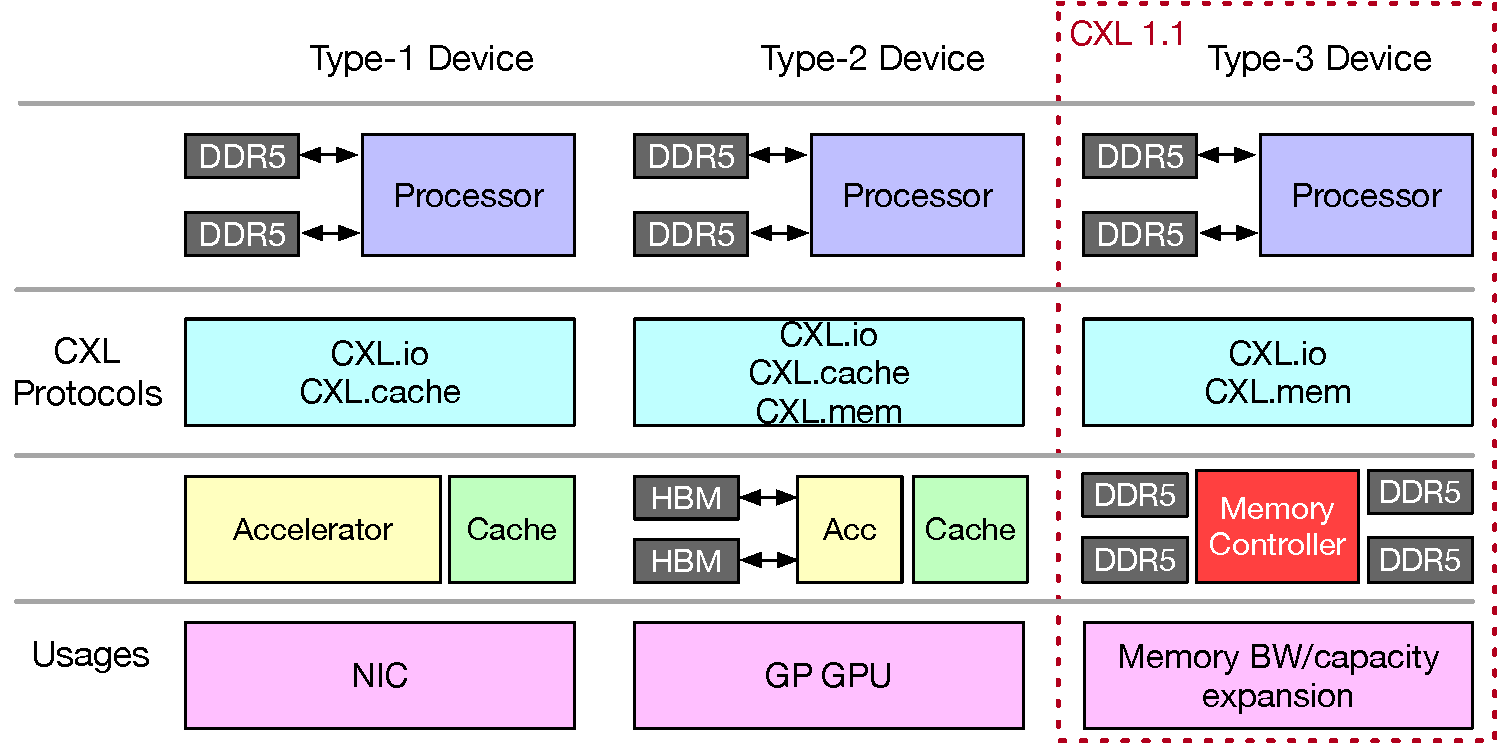
\includegraphics[width=\textwidth]{cxl}
      \caption{\textbf{CXL Overview}} 
    \label{fig:cxl} \vspace{-1.0em}
    \end{figure*}

\begin{figure}[t]
    \centering
      \includegraphics[width=0.9\columnwidth]{cxl_performance}\vspace{-1.0em}
      \caption{\textbf{CXL Performance for Read-only Workload.} CXL denotes accessing memory through Compute Express Link, while DRAM refers to traditional memory access. The '-r' suffix indicates remote socket access.} \vspace{-2.0em}
    \label{fig:cxlperformance}
    \end{figure}
    
\end{comment}
While network-based resource disaggregation has gained attention due to advancements in network bandwidth (\S\ref{sec:os}), the inherent latency, limited by the speed of light, still imposes significant overheads. This section explores the potential of next-generation interconnects and their impact on resource disaggregation.

\section{Next-generation Interconnects}

Recent advancements in hardware have led to the development of new-generation interconnects by major hardware vendors, such as NVLink~\cite{nvlink} from Nvidia and Compute Express Link (CXL)~\cite{cxl} from Intel. CXL, in particular, has been introduced as a promising solution to expand memory capacity and bandwidth by attaching external memory devices to PCIe slots, offering a dynamic and heterogeneous computing environment.

\paragraphb{Compute Express Link (CXL)}
As depicted in Figure~\ref{fig:cxl}, CXL encompasses three key protocols: CXL.mem, CXL.cache, and CXL.io. CXL.io serves as the PCIe physical layer. CXL.mem enables processors to access memory over PCIe, while CXL.cache facilitates coherent memory access between processors and accelerators. These protocols allow for the construction of various CXL device types. The initial CXL 1.1 version serves as a memory expander for a single server. Subsequent versions, like CXL 2.0, extend this capability to multiple servers, incorporating CXL switches that coordinate access from different servers and enable various compute nodes to share a large memory pool. The forthcoming CXL 3.0 aims to scale up further, with cache coherency managed by hardware.

Despite extensive research on CXL~\cite{cxl_azure,cxlcentric,demystify}, practical, commercial CXL hardware implementations remain in development, posing challenges in fully understanding performance and system support design for such hardware. Most studies have relied on simulations or FPGA-based CXL hardware~\cite{demystify,intelfpga}, lacking empirical evaluations on ASIC-based CXL hardware. Moreover, existing research often focuses on single aspects of CXL, like capacity or bandwidth, using synthetic benchmarks and neglecting a comprehensive evaluation that includes cost considerations. To gauge the performance of real CXL hardware and assess its suitability for resource disaggregation, we evaluated the latest hardware available: Intel's $\text{4}^{th}$ generation scalable processor (Sapphire Rapids) and Asteralabs's CXL 1.1 memory expander (Type-3 device). Using Intel Memory Latency Checker (MLC)\cite{mlc}, we measured the latency of reading data from the CXL device and local memory equipped with the same amount of DDR5 channels for local and cross-socket access. Figure\ref{fig:cxlperformance} reveals that the latest CXL hardware exhibits a latency of more than $2.5\times$ higher than local memory. However, this gap narrows for cross-socket access, suggesting CXL as another memory tier. This raises questions about whether and how this information should be exposed to applications. Previous research~\cite{tpp} has investigated promoting hot pages from slower-tiered memory at the kernel level to enhance performance while maintaining application transparency.

This study represents the first available evaluation of real CXL 1.1 ASICs. The performance of CXL 2.0 and 3.0 remains to be explored in future work.

\subsection{Introduction}
\subsection{Background and Methodology}
\subsection{CXL 1.1 Performance characteristics}
\subsection{Memory Capacity-bound Applications}

\subsection{Memory Bandwidth-bound Applications}

\subsection{Cost Implications}

\subsection{Discussion and Conclusion}
